\section{Laufzeitvergleiche}
Zur Feststellung der Effizienz unserer Parallelisierungen haben wir die Laufzeit des Programms mit verschiedenen Parametern
aufgezeichnet. Um vergleichbare Ergebnisse zu erhalten, wurden alle Messungen mit einem festen Winkel von 30° und gleichen Höhen
(Höhe = Länge = Breite des Würfels mit einem Startwürfel der Seitenlänge 2) durchgeführt. 
Die Baumtiefe --- und damit die Anzahl zu berechnender Würfel --- wurde durch die Anzahl an Ebenen variiert.\\
Jeder Messwert in den folgenden Diagrammen wurde auf allen Geräten durch siebenfache Programmausführung und anschließendes
Bilden des Mittelwerts bestimmt (siehe \hyperref[Anhang]{Anhang}). Zur besseren Veranschaulichung wurden die Graphen in zwei Abschnitte unterteilt --- der 
erste Teil zeigt das Verhalten bei geringen Baumtiefen von fünf bis 13 Ebenen, der zweite Abschnitt für größere
Baumtiefen von 15 bis 21 Ebenen.

\vspace{-0.25cm}
\subsection{Sequentiell vs. OpenCL}
\vspace{-0.25cm}
Die folgenden Diagramme vergleichen die Laufzeit einer sequentiellen Ausführung mit einer durch OpenCL 
parallelisierten Ausführung.\\
Auf dem Thinkpad P15 wurde mit OpenCL je nach Baumtiefe eine Beschleunigung von etwa 40\% bis 87\% erreicht.
Allerdings trat diese erst bei Bäumen mit mehr als 16 Ebenen ein. Für Bäume mit nur fünf bis sieben Ebenen war OpenCL um 
den Faktor 120 - 360 langsamer als das sequentielle Pendant. 
\begin{figure}[H]
    \centering
    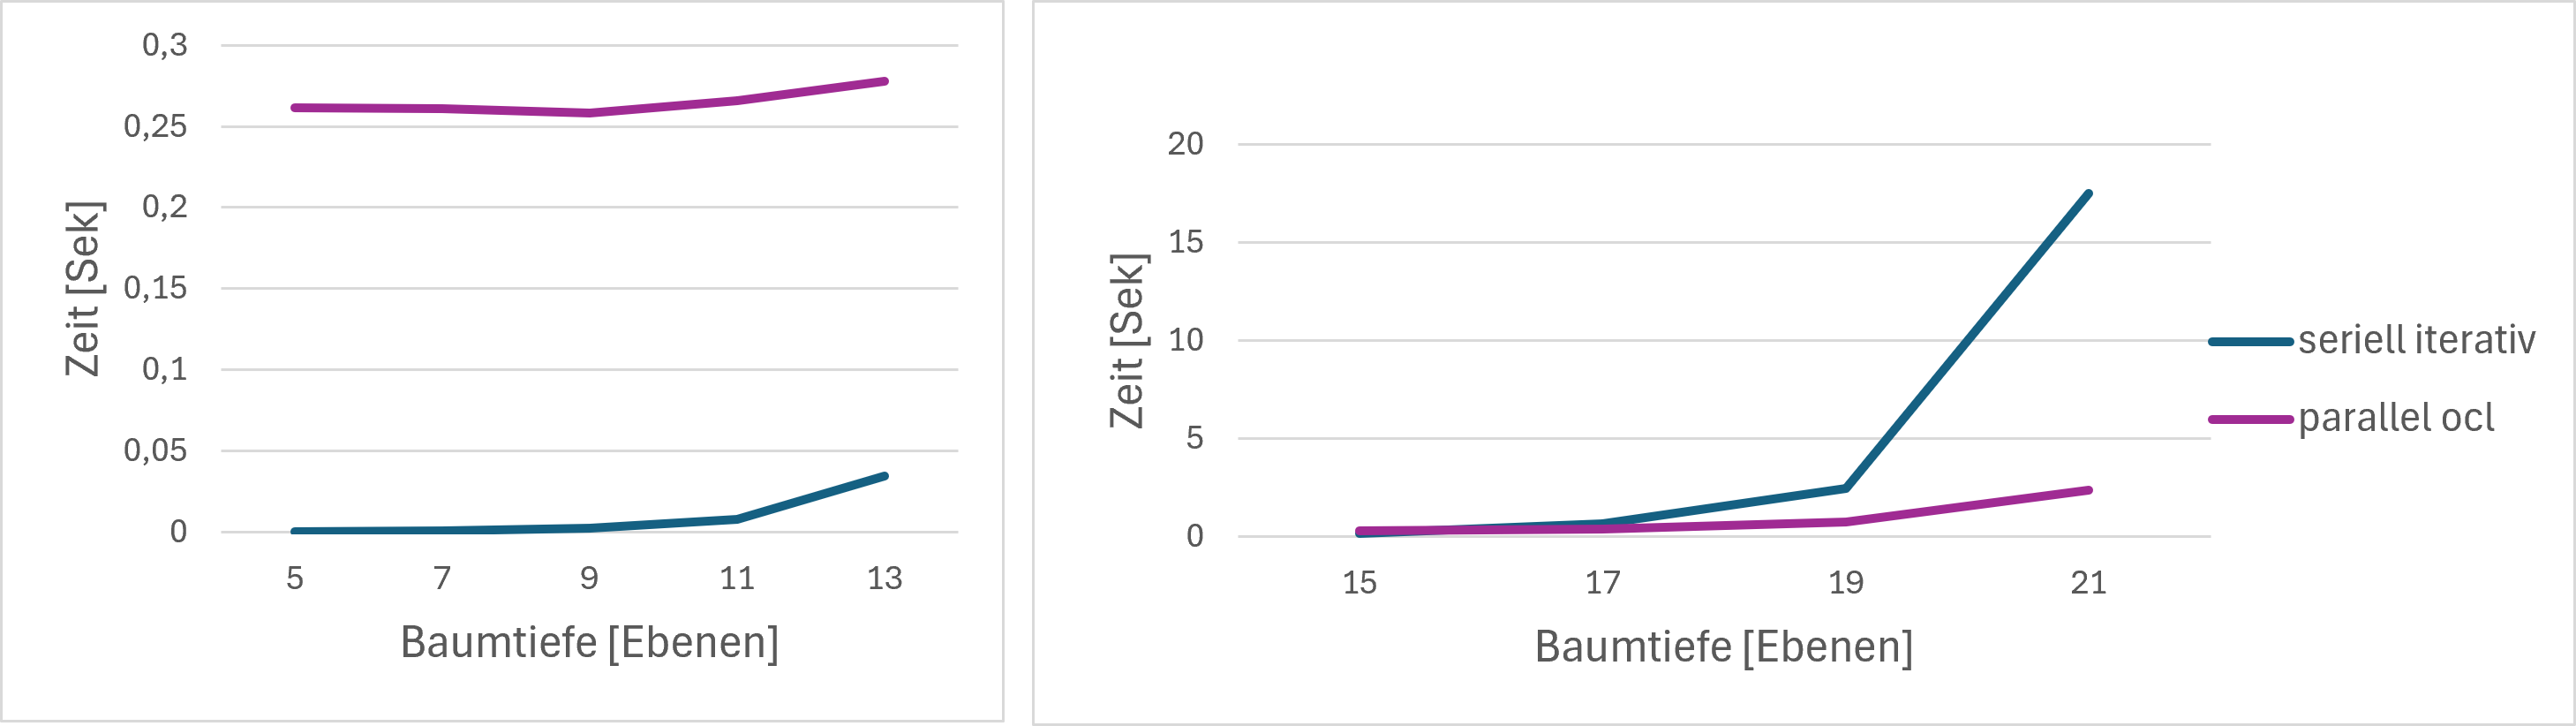
\includegraphics[width=0.9\linewidth]{./diagrams/seriellVsOCL_Tomke.png}
    \caption{Vergleich sequentielle vs. OpenCL Ausführung auf Thinkpad P15 Gen 2}
    \label{fig:seriellOCL1}
\end{figure}

\noindent Auf dem ASUS ZenBook war die OpenCL-Implementierung besonders für geringe Baumtiefen
ebenfalls deutlich im Nachteil. Für mittelgroße Bäume mit elf bis 17 Ebenen brauchte OpenCL etwa 2,5 bis 85x so 
lange wie die sequentielle Ausführung, bei sehr kleinen Bäume sogar zwischen etwa 300 und 
4000 Mal länger.
Erst ab einer Größe von 21 Ebenen zeigte sich ein Vorteil durch die Parallelisierung auf der GPU.
\begin{figure}[H]
    \centering
    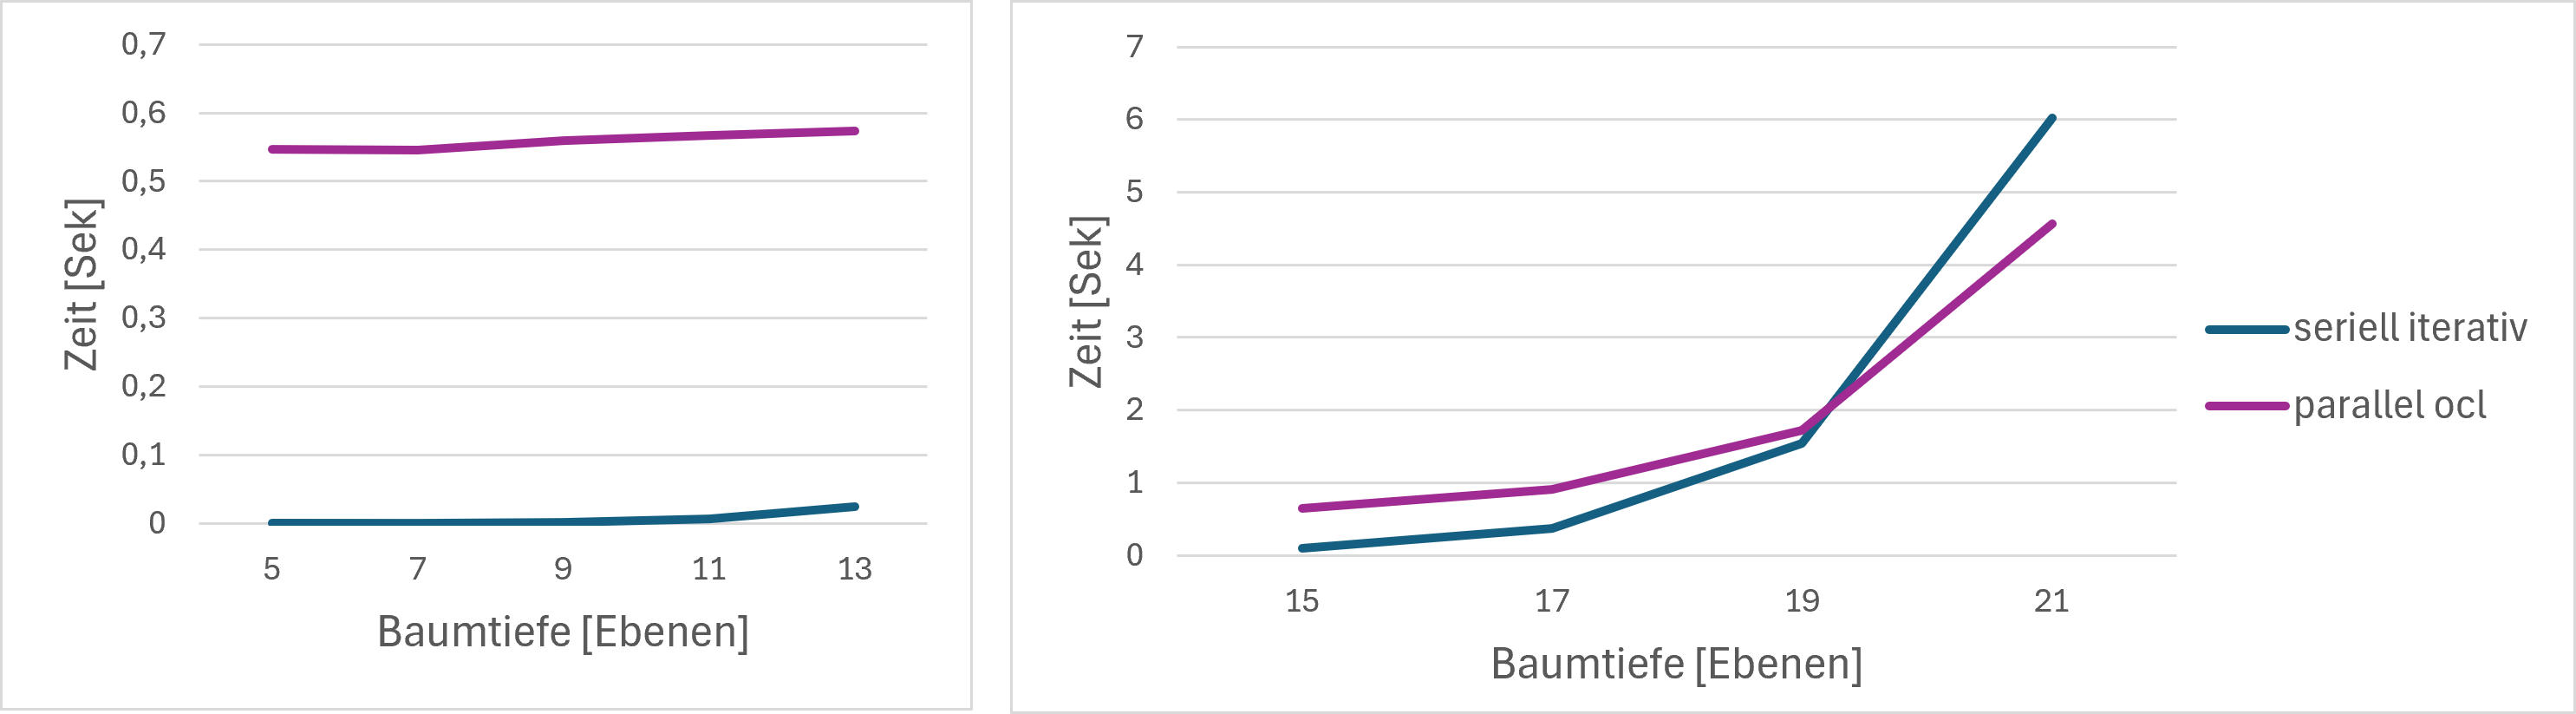
\includegraphics[width=0.9\linewidth]{./diagrams/seriellVsOCL_Sofie.png}
    \caption{Vergleich sequentielle vs. OpenCL Ausführung auf ASUS ZenBook 13}
    \label{fig:seriellOCL2}
\end{figure}

\noindent Anders als auf den anderen beiden Geräten war die Ausführung mit OpenCL auf dem Thinkpad P14s schon 
ab 15 Ebenen Baumtiefe deutlich schneller als die sequentielle Implementierung. Insgesamt konnte eine
Beschleunigung von 35\% - 88\% erreicht werden. Selbst für geringere Baumtiefen war die OpenCL-Ausführung im 
Vergleich zu der Ausführung auf den zuvor betrachteten Geräten schneller. Dennoch war OpenCL etwa 2x bis 375x 
langsamer als die sequentielle Implementierung.
\begin{figure}[H]
    \centering
    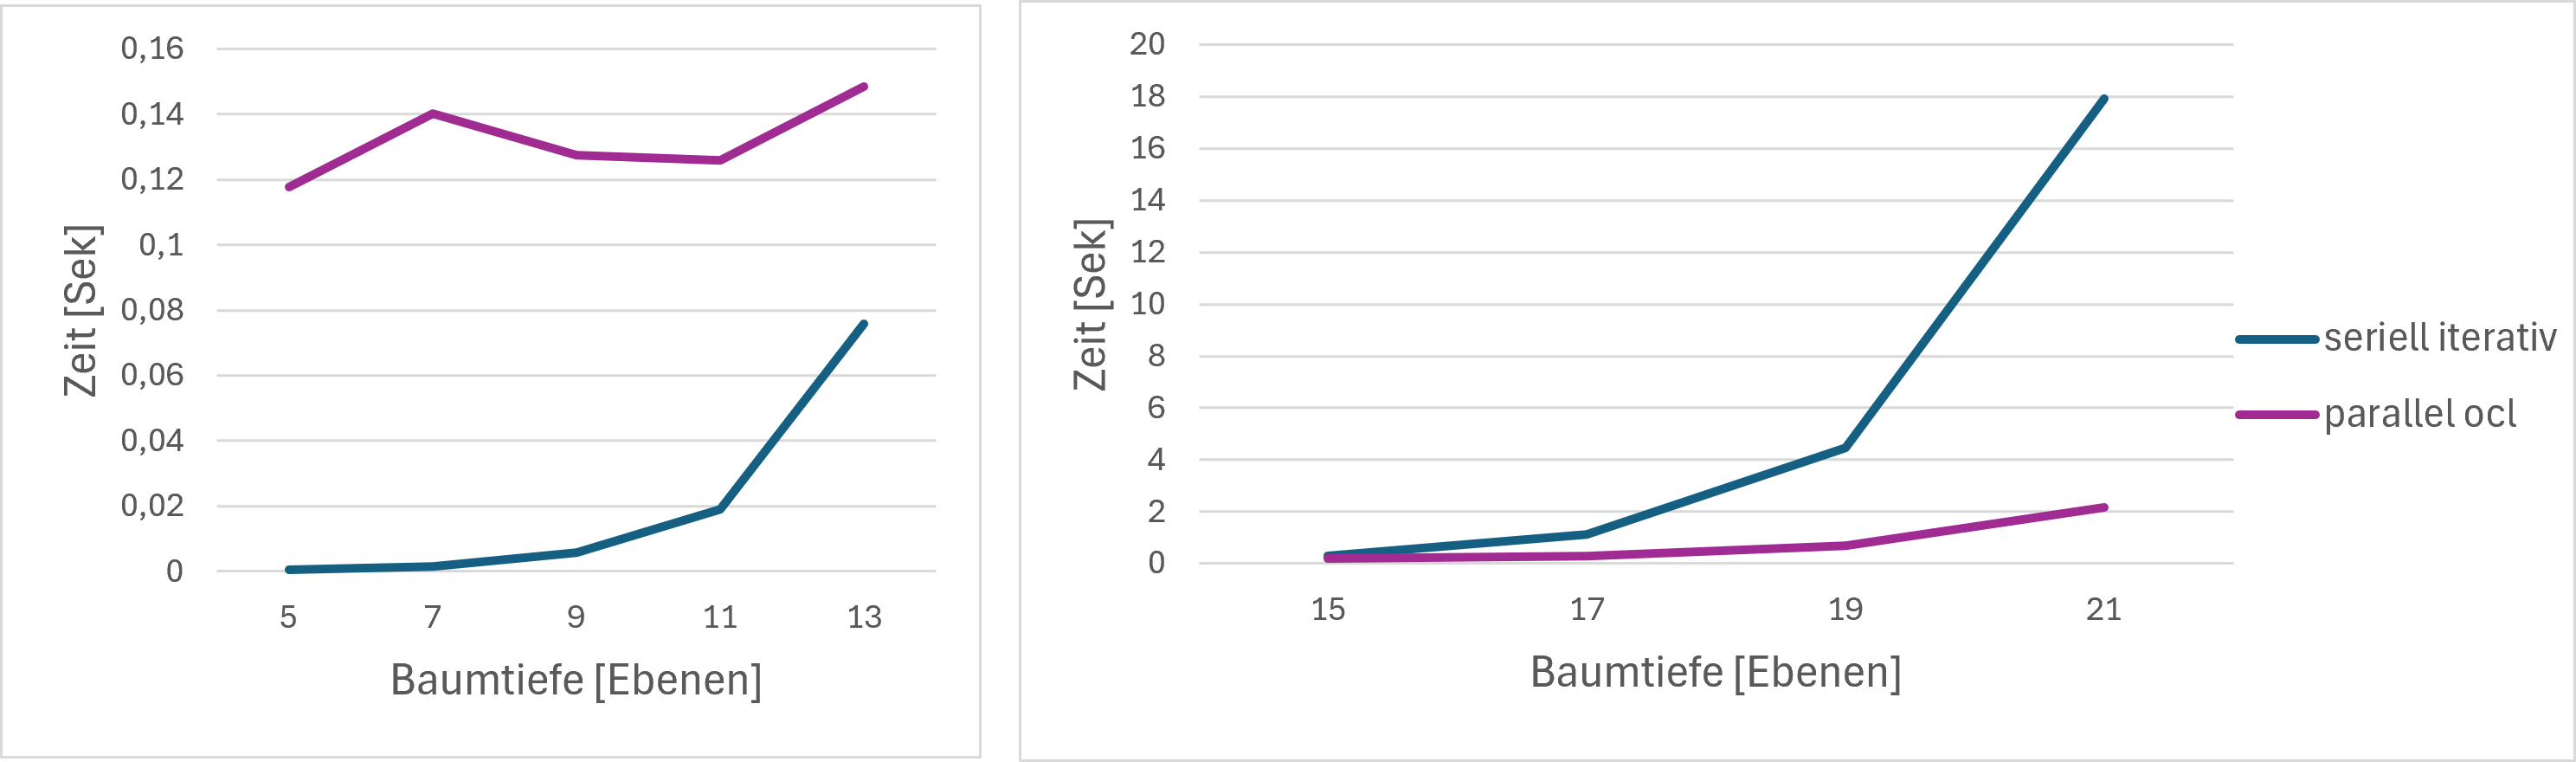
\includegraphics[width=0.9\linewidth]{./diagrams/seriellVsOCL_Patrick.png}
    \caption{Vergleich sequentielle vs. OpenCL Ausführung auf Thinkpad P14s Gen 1}
    \label{fig:seriellOCL3}
\end{figure}

\subsection{Sequentiell vs. OpenMP}
\vspace{-0.25cm}
Im nächsten Schritt haben wir die Ausführungszeiten unserer sequentiellen Implementierung denen der Parallelisierung
mit OpenMP gegenübergestellt.\\
Hierbei war OpenMP auf dem Thinkpad P15 für Bäume mit fünf bis sieben Ebenen zwar etwa doppelt so langsam wie die sequentielle 
Implementierung, konnte die Ausführung bei Bäumen mit elf oder mehr Ebenen aber zwischen 50\% und 93\% Zeitersparnis erwirken.
\begin{figure}[H]
    \centering
    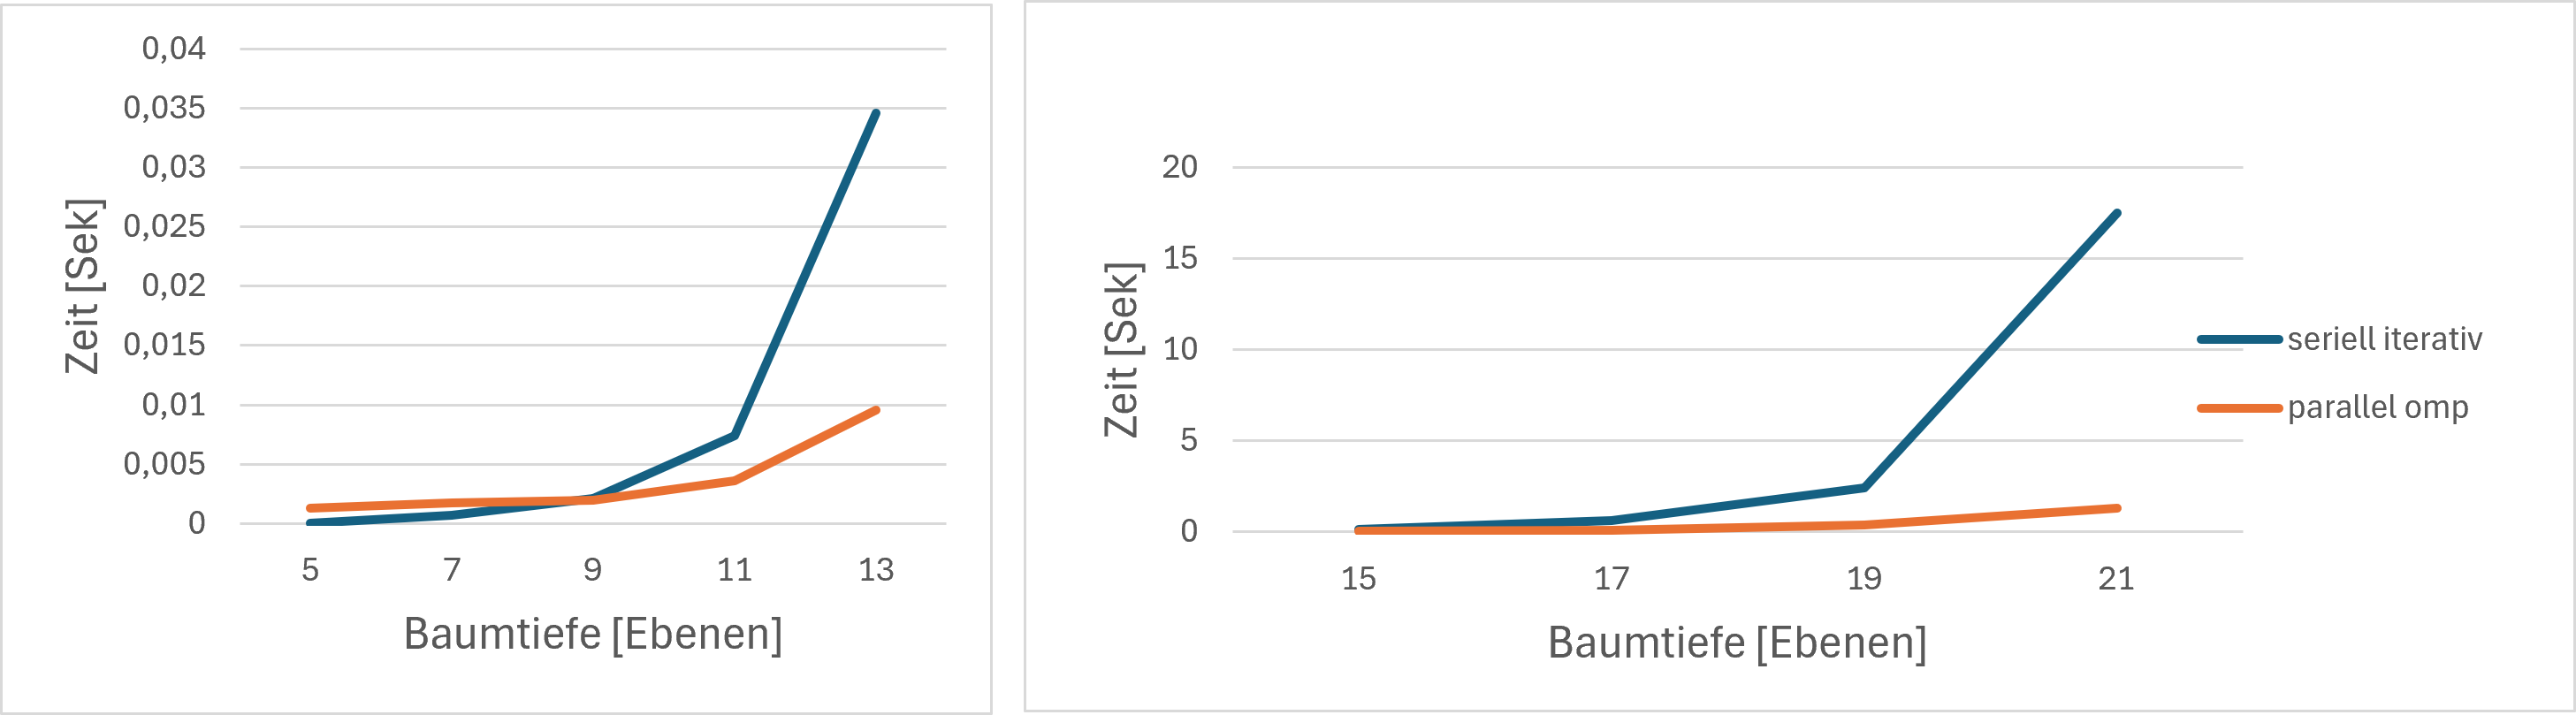
\includegraphics[width=\linewidth]{./diagrams/seriellVsOMP_Tomke.png}
    \caption{Vergleich sequentielle vs. OpenMP Ausführung auf Thinkpad P15 Gen 2}
    \label{fig:seriellOMP1}
\end{figure}

\noindent Auch auf dem ASUS ZenBook konnte ab elf Ebenen Baumtiefe eine Beschleunigung von 50\% festgestellt werden. Die höchste 
Zeitersparnis lag bei 80\%. Für kleine Bäume war die sequentielle Implementierung um einen Faktor von 1,5 bis 6 zeiteffizienter.
\begin{figure}[H]
    \centering
    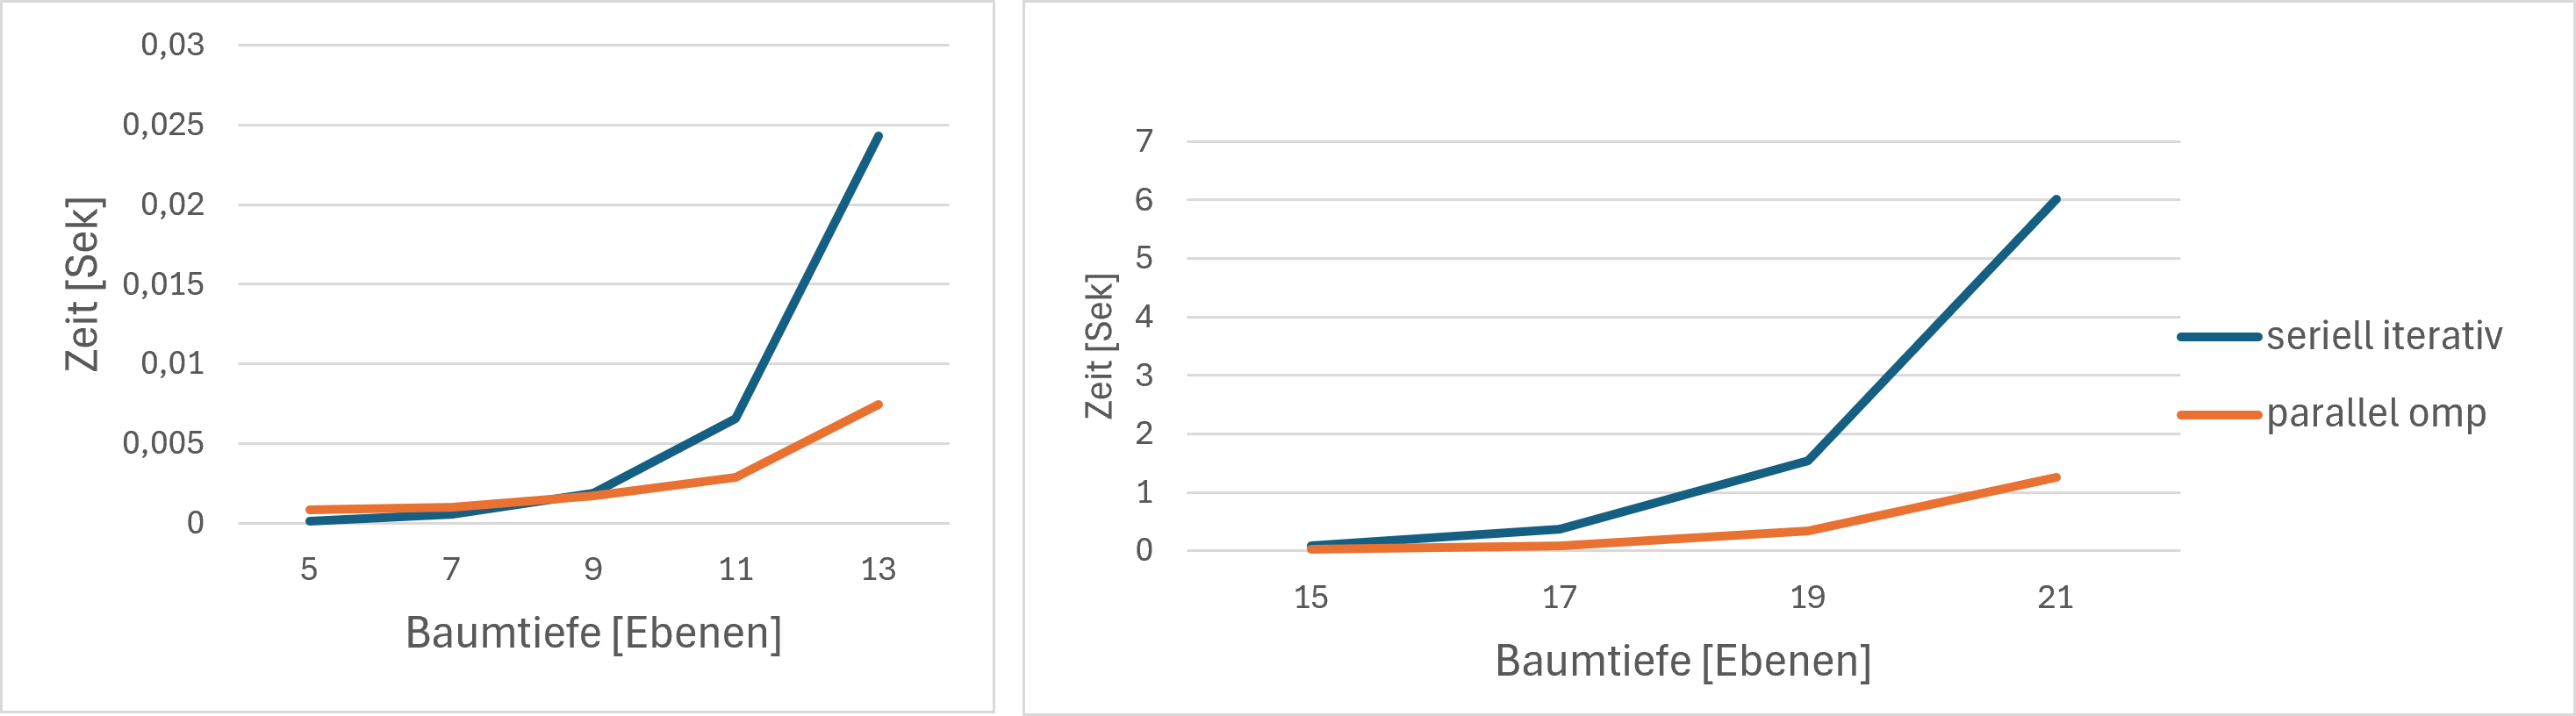
\includegraphics[width=\linewidth]{./diagrams/seriellVsOMP_Sofie.png}
    \caption{Vergleich sequentielle vs. OpenMP Ausführung auf ASUS ZenBook 13}
    \label{fig:seriellOMP2}
\end{figure}

\noindent Deutlich schlechter waren die für OpenMP gemessenen Zeiten für kleine Bäume auf dem Thinkpad P14s. Hier war die sequentielle Ausführung 
zwischen drei und 30x schneller. Dafür konnte eine Beschleunigung mit Faktor zwei durch die Parallelisierung schon bei neun Ebenen 
erwirkt werden. Insgesamt war eine Beschleunigung von bis zu 80\% möglich.
\begin{figure}[H]
    \centering
    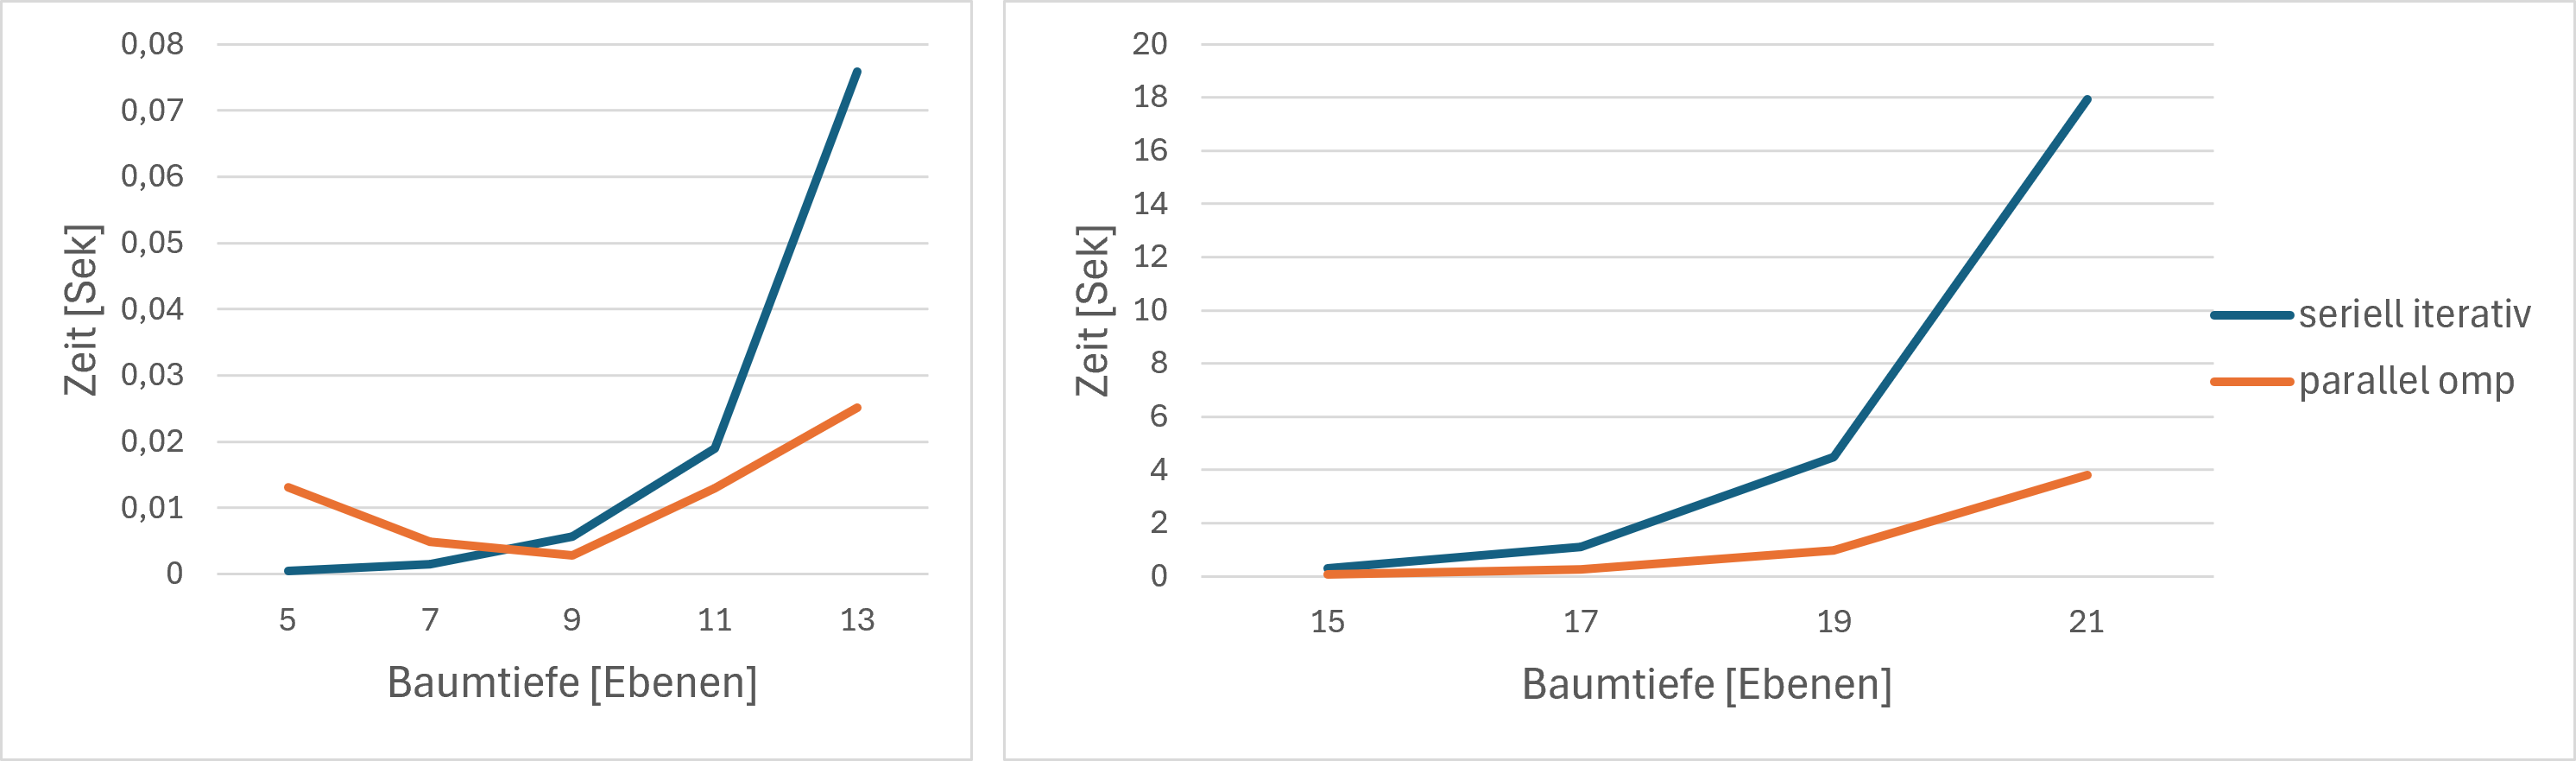
\includegraphics[width=\linewidth]{./diagrams/seriellVsOMP_Patrick.png}
    \caption{Vergleich sequentielle vs. OpenMP Ausführung auf Thinkpad P14s Gen 1}
    \label{fig:seriellOMP3}
\end{figure}

\subsection{OpenCL vs. OpenMP}
\vspace{-0.25cm}
Um einen Eindruck über die bestmögliche Beschleunigung unseres Programms zu gewinnen, haben wir zuletzt auch die beiden parallelen 
Technologien, OpenCL und OpenMP, gegenübergestellt.\\
Während auf dem Thinkpad P15 und dem ASUS ZenBook OpenCL deutlich langsamer war als OpenMP --- Faktoren zwischen 2 und 630 --- war
auf dem Thinkpad P14s ab 19 Ebenen OpenCL um 30 - 45\% schneller.
\vspace{0.5cm}\\
\begin{minipage}{0.49\linewidth}
    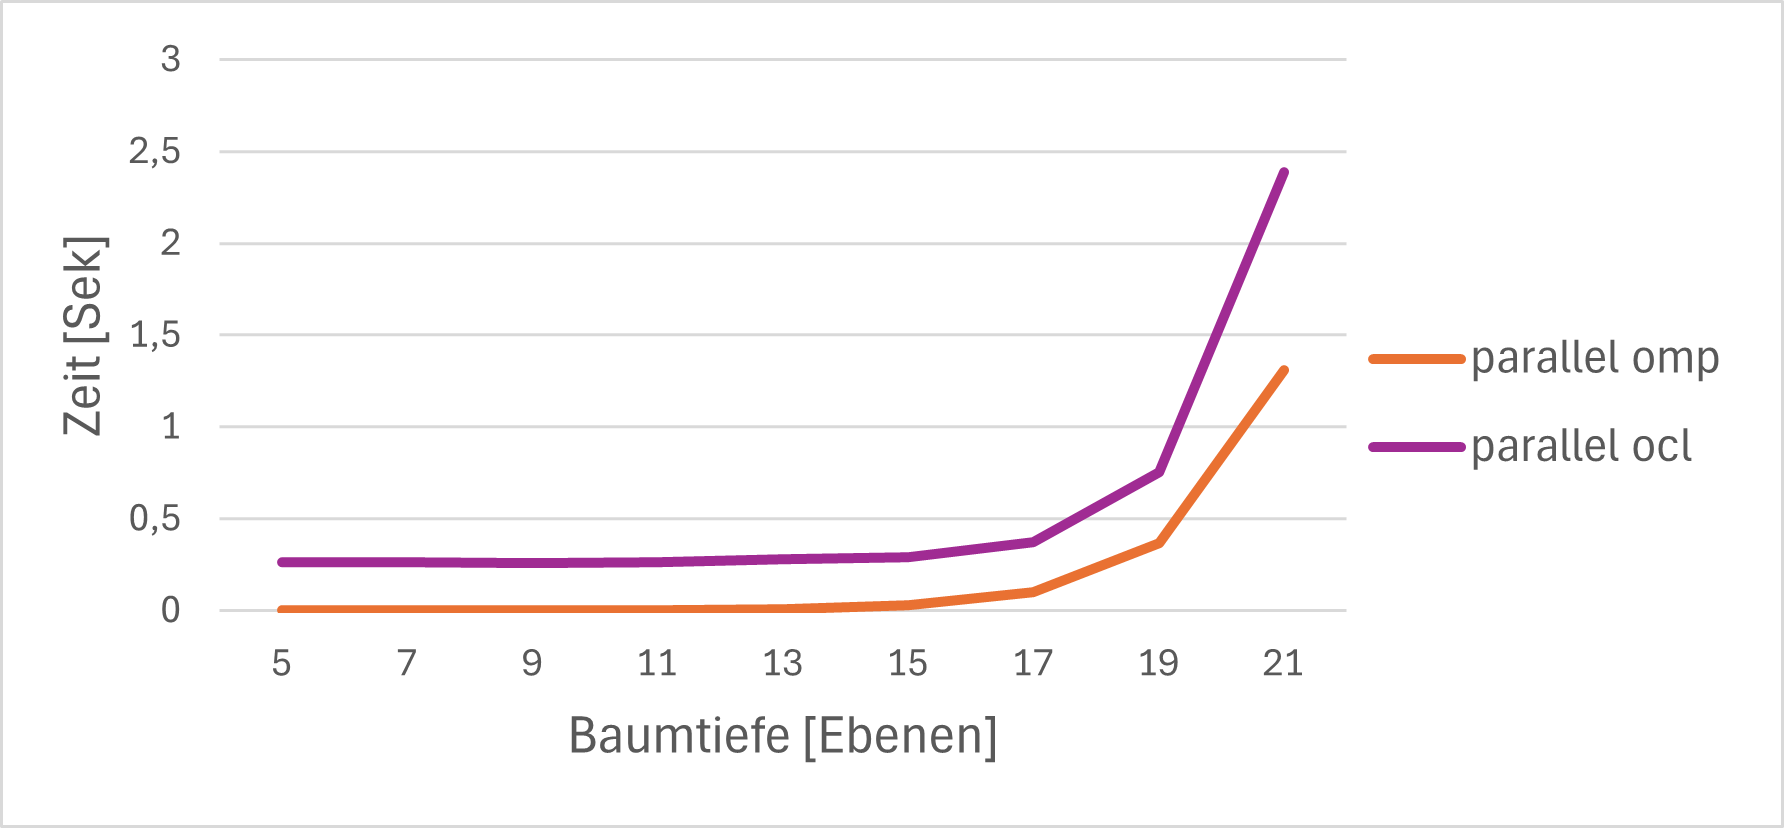
\includegraphics[width=\linewidth]{./diagrams/ompVsOCL_Tomke.png}
    \captionof{figure}{Vergleich OpenMP vs. OpenCL Ausführung auf Thinkpad P15 Gen 2}
    \label{fig:ocl-opm-1}
\end{minipage}
\hfill
\begin{minipage}{0.49\linewidth}
    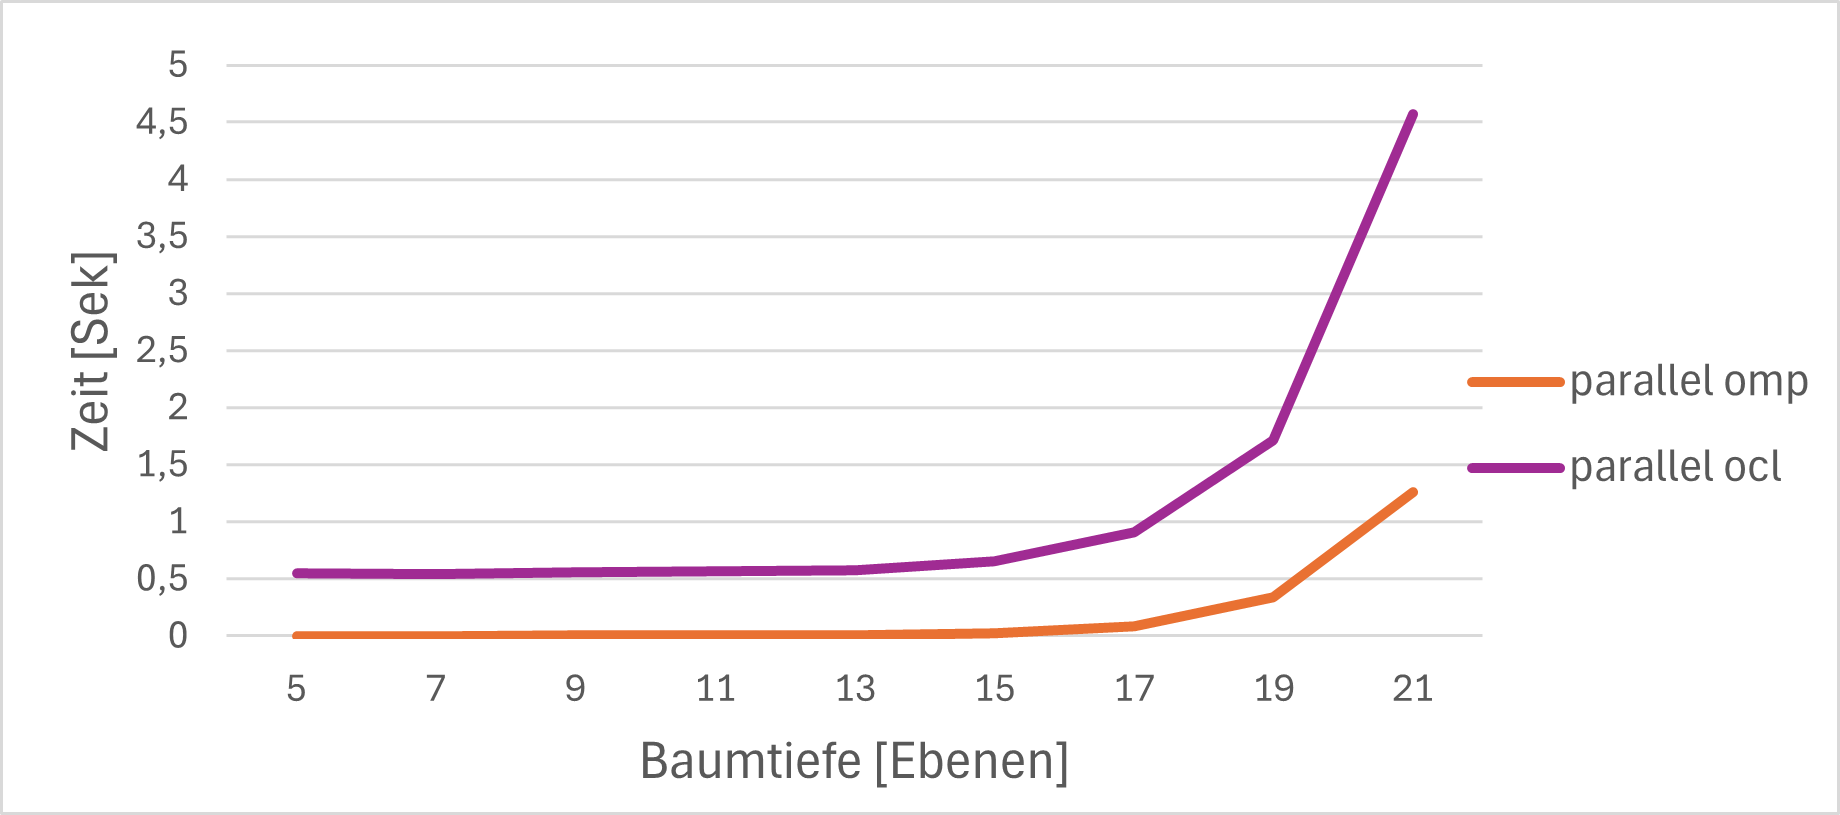
\includegraphics[width=\linewidth]{./diagrams/ompVsOCL_Sofie.png}
    \captionof{figure}{Vergleich OpenMP vs. OpenCL Ausführung auf ASUS ZenBook 13}
    \label{fig:ocl-opm-2}
\end{minipage}
\begin{figure}[H]
    \centering
    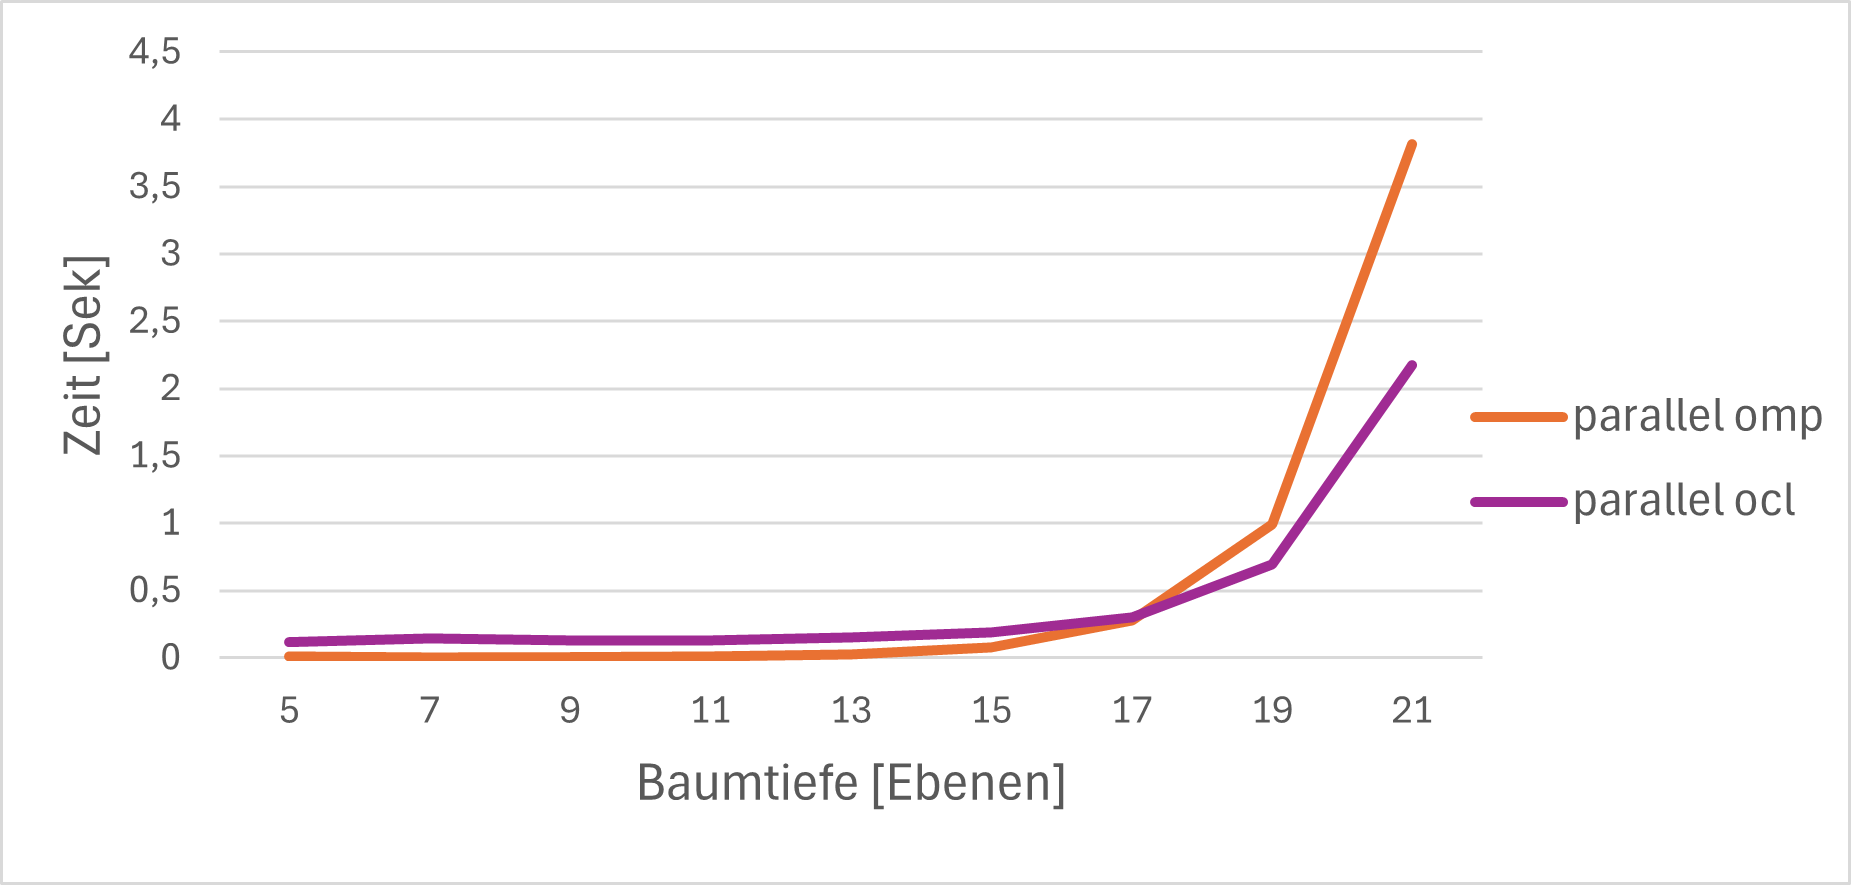
\includegraphics[width=0.5\linewidth]{./diagrams/ompVsOCL_Patrick.png}
    \caption{Vergleich OpenMP vs. OpenCL Ausführung auf Thinkpad P14s Gen 1}
    \label{fig:ocl-opm-1}
\end{figure}

\vspace{0.25cm}
\noindent Der erhebliche zeitliche Nachteil, welchen OpenCL vor allem bei geringen Baumtiefen aufweist, lässt
sich durch den Overhead erklären der entsteht, weil die zu verarbeitenden Daten --- das Array mit den Quadern --- über
den Systembus aus dem Arbeitsspeicher der CPU in den Grafikkarteneigenen RAM kopiert werden müssen.\\
Hiermit ist auch zu begründen, dass die für die OpenCL-Ausführung gemessenen Zeiten auf dem Thinkpad P14s deutlich schneller
sind. Durch die Verwendung von PoCL müssen die Daten nur innerhalb der CPU kopiert werden, was eine erhebliche Zeitersparnis 
mit sich bringt.

\vspace{0.5cm}
\begin{minipage}{0.49\linewidth}
    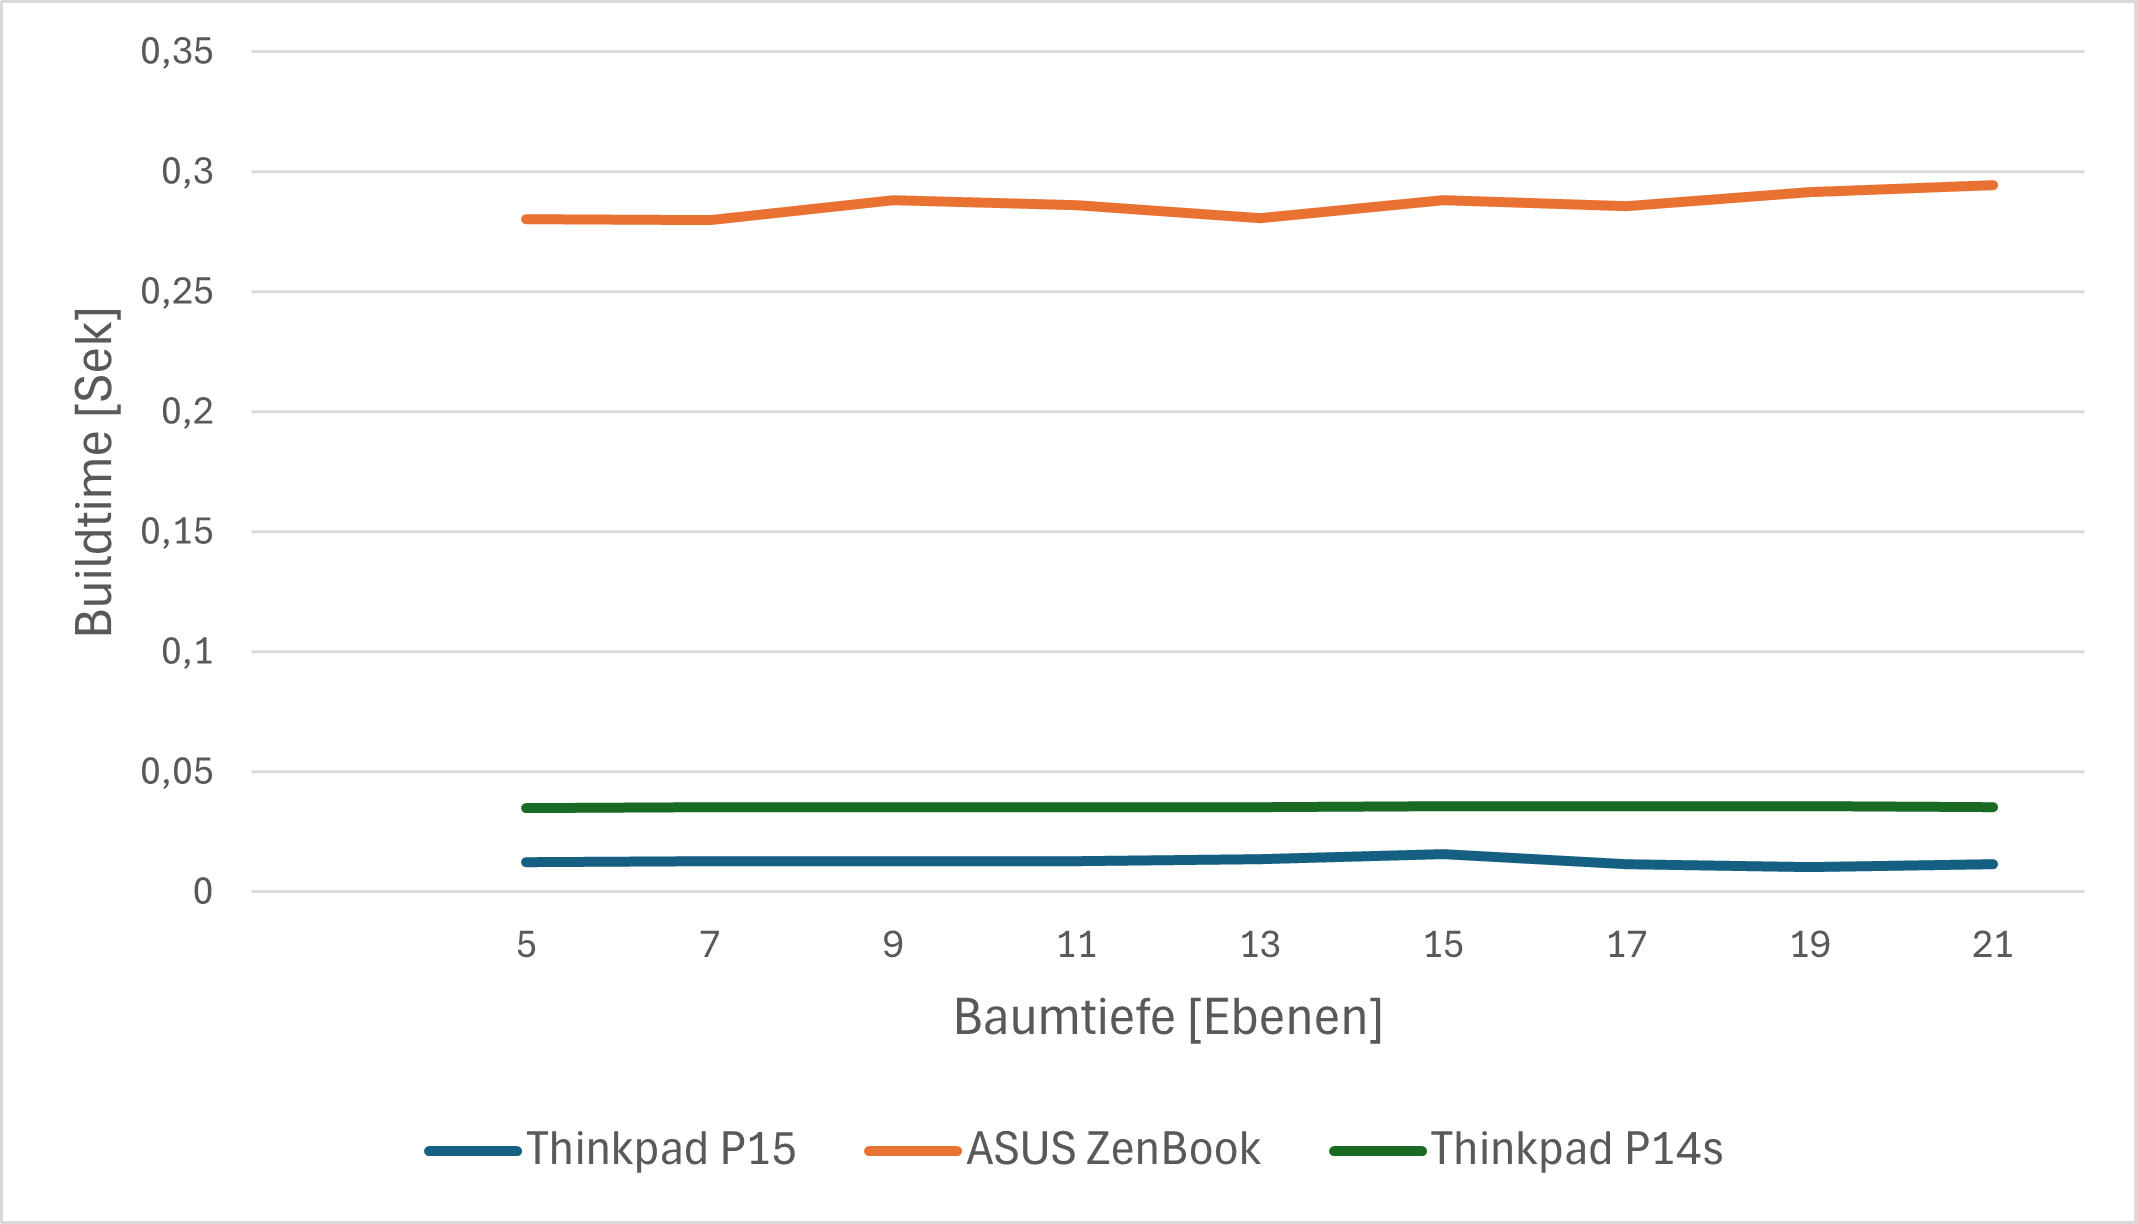
\includegraphics[width=\linewidth]{diagrams/OpenCL_Buildtime.png}
    \captionof{figure}{Buildzeit OpenCL-Kerlen auf verschiedenen Rechnern}
\end{minipage}
\hfill
\begin{minipage}{0.49\linewidth}
    Ein wichtiger Einflussfaktor auf die Laufzeit von OpenCL ist die Zeit, die für den Kernel-Bau vonnöten ist. 
    Die obigen Diagramme zeigen die Ausführungszeit bereits kompilierten Codes. 
    Wie das Diagramm links abbildet, ist die Buildtime weitgehend unabhängig von der Baumtiefe, variiert jedoch je nach 
    Rechner --- auf schnellen Systemen liegt sie unter 0,015 Sekunden, auf langsameren unter 0,3 Sekunden. 
\end{minipage} 

% ----------------------------------- Auslastung CPU / Speicher -----------------------------------
% -------------------------------------------------------------------------------------------------
\vspace{0.25cm}
\subsection{Auslastung von CPU und Speicher}\label{Speicher}
\vspace{-0.25cm}
Um sicherzustellen, dass --- besonders bei der parallelen Implementierung mit OpenMP --- die CPU tatsächlich 
ausgelastet wird, haben wir die Auslastung der CPU und des Speichers während der Programmausführung überwacht.

\begin{figure}[!ht]
    \centering
    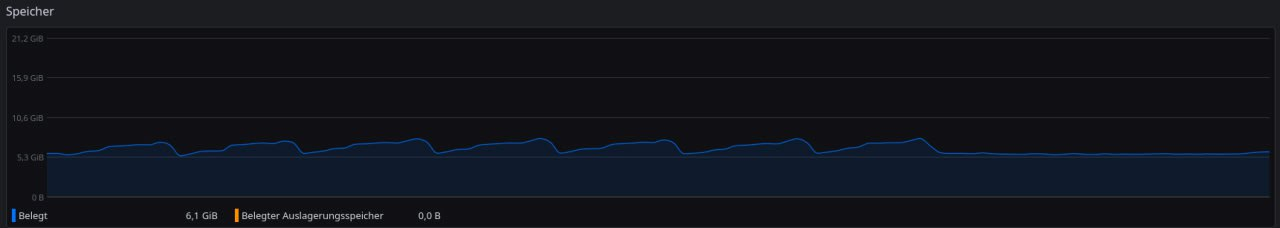
\includegraphics[width=\linewidth]{./diagrams/Memory.jpg}
    \caption{Auslastung des RAM eines Thinkpad P14s Gen 1 während der Programmausführung}
    \label{fig:memory}
\end{figure}
\vspace{-0.25cm}
\noindent Grafik~\ref{fig:memory} zeigt die RAM-Auslastung eines Thinkpad P14s Gen 1 während eines Programmlaufs. 
Dabei entspricht ein Intervall der Kurve, in welchem der Graph bis zu einem Hochpunkt steigt und anschließend auf 
einen Tiefpunkt abfällt, einer Programmausführung.\\
Die Auslastung des RAMs war bei allen Arten der Implementierung (seriell iterativ, parallel mit OpenMP, parallel 
mit OpenCL) sehr ähnlich.

\vspace{0.5cm}
\begin{figure}[!ht]
    \centering
    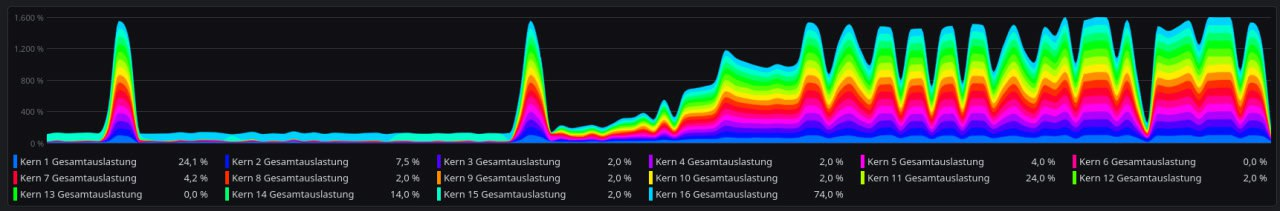
\includegraphics[width=\linewidth]{./diagrams/Serial-OpenMP.jpg}
    \caption{CPU-Auslastung im Übergang von sequentieller zu paralleler Berechnung mit OpenMP}
    \label{fig:Serial-OpenMP}
\end{figure}
\vspace{-0.25cm}
\noindent In Grafik~\ref{fig:Serial-OpenMP} ist die CPU-Auslastung während eines Programmlaufs mit anfangs sequentieller 
und später CPU-paralleler Ausführung zu sehen.\\
Die einzelnen Hochpunkte des Graphen in der ersten Hälfte des Diagrams kommen zustande, weil das Hinzufügen der
Quadern zum Renderer mit OpenMP parallelisiert erfolgt, um eine optimale Ausführungszeit gewährleisten zu können.
Die entsprechende Funktion \texttt{addRenderObject()} ist im Renderer angesiedelt und für alle unsere Implementierungen 
gleich.\\
Zu sehen ist auch, dass erst bei späten Baumtiefen eine Auslastung mehrerer Kerne erreicht wird. 

\vspace{0.5cm}
\begin{figure}[!ht]
    \centering
    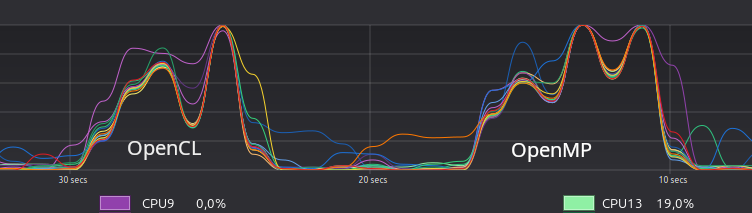
\includegraphics[width=0.9\linewidth]{./diagrams/OpenCL-OpenMP.png}
    \caption{CPU-Auslastung OpenCL im Vergleich zu OpenMP}
    \label{fig:CPU-OpenCL-OpenMP}
\end{figure}
\vspace{-0.25cm}
\noindent
Wie Grafik~\ref{fig:CPU-OpenCL-OpenMP} zeigt, ist die CPU-Auslastung bei einer parallelisierten Ausführung mit 
einer Baumtiefe von 21 Ebenen bei OpenCL minimal geringer als bei OpenMP --- jedoch deutlich weniger, als zu erwarten war. 
Dies ist damit zu begründen, dass die Berechnung der Quader auf der GPU erfolgt, das Übertragen der Daten an den
Renderer aber auf der CPU stattfindet. Während diese Weiterverarbeitung der generierten Daten in der seriellen Implementierung bis 
auf die letzte Ebene seriell ausgeführt wird, ist sie bei der OpenCL-Implementierung mit OpenMP parallelisiert, um eine Verunreinigung
der Zeitmessungen durch den Renderer möglichst gering zu halten. Einen nicht zu vernachlässigenden Rechenaufwand stellt dabei das 
Überführen der von der GPU zurückgelieferten Werte in ein vom Renderer anzeigbares Format.\\

\vspace{0.5cm}
\begin{figure}[!ht]
    \centering
    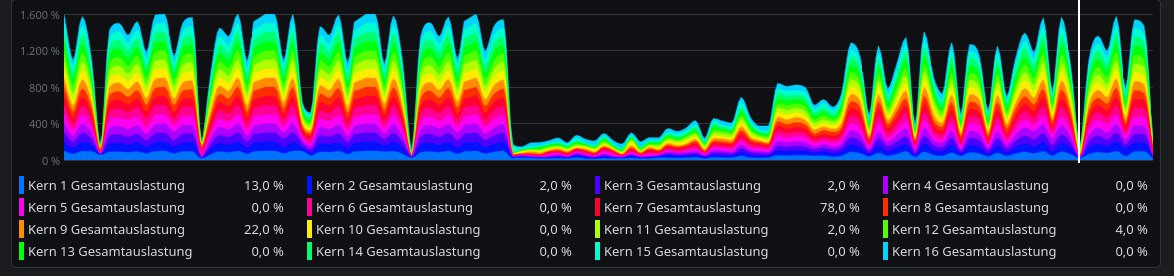
\includegraphics[width=0.9\linewidth]{./diagrams/OpenMP-OpenCL-POCL.jpg}
    \caption{CPU-Auslastung bei paralleler Programmausführung mit Übergang von OpenMP zu OpenCL}
    \label{fig:OpenMP-OpenCL}
\end{figure}

\noindent
Grafik \ref{fig:OpenMP-OpenCL} bildet die CPU-Auslastung während eines parallelen Programmablaufs ab, bei welchem 
zuerst mit OpenMP und danach mit OpenCL gearbeitet wird. Wie gut zu erkennen ist, ist die CPU-Auslastung für große Baumtiefen während beider Ausführungen bei allen Kernen 
vergleichsweise hoch, was darauf zurückzuführen ist, dass aus \hyperref[Hardware]{hardwaretechnischen Gründen} auch die OpenCL-Implementierung
auf der CPU ausgeführt wird.\\
Interessant ist, dass in diesem Fall die CPU-Auslastung mit OpenCL augenscheinlich geringer war, während die Laufzeit dennoch niedriger
blieb. Der Abschnitt hinter der in der Grafik eingezeichneten weißen Linie zeigt eine Ausführung des Programms mit 21 Ebenen unter 
Verwendung von OpenCL, also ebenso wie die letzten Ausführungen unter Verwendung von OpenMP. \\

% ----------------------------------- Beschleunigung (Amdahl) -----------------------------------
% -----------------------------------------------------------------------------------------------
\subsection{Beschleunigungsfaktor nach Amdahl}
\flushleft Zur Bestimmung des Beschleunigungsfaktors nach Amdahl erfassten wir einmalig die serielle Ausführungszeit (SERT) und 
gleichzeitig die Laufzeit des parallelisierbaren Codes (PT). Aus diesen \hyperref[Anhang]{Messwerten} berechneten wir die benötigten Parameter
\vspace{0.15cm}\\
\centering $P = PT / SERT$ und $S = (SERT - PT) / SERT$ 
\vspace{-0.15cm}
\flushleft sodass wir letztendlich für die verschiedenen Baumtiefen die Beschleunigungsfaktoren kalkulieren konnten:
\begin{table}[H]
    \centering
    \small
    \begin{tabular}{@{}cccccc@{}}
        \toprule
        Baumtiefe & P        & N    & S         & Beschleunigungsfaktor \\ \midrule
        1         & 0.333   & 4096 & 1.000     & 1.500 \\
        2         & 0.000   & 4096 & 0.667     & 1.000 \\
        3         & 0.000   & 4096 & 3.334     & 5.999 \\
        4         & 0.286   & 4096 & 0.714     & 5.993 \\
        5         & 0.000   & 4096 & 4.286     & 7.190 \\
        6         & 0.913   & 4096 & 0.728     & 3.999 \\
        7         & 0.000   & 4096 & 5.000     & 8.524 \\
        8         & 0.000   & 4096 & 2.157     & 3.037 \\
        9         & 0.000   & 4096 & 6.205     & 9.867 \\
        10        & 0.995   & 4096 & 0.722     & 5.156 \\
        11        & 0.895   & 4096 & 0.712     & 5.966 \\
        12        & 0.835   & 4096 & 0.361     & 3.021 \\
        13        & 0.892   & 4096 & 0.719     & 6.234 \\
        14        & 0.899   & 4096 & 0.861     & 6.635 \\
        15        & 0.821   & 4096 & 0.814     & 6.996 \\
        16        & 0.000   & 4096 & 8.575     & 12.756 \\
        17        & 0.000   & 4096 & 0.686     & 5.581 \\
        18        & 0.000   & 4096 & 0.838     & 7.648 \\
        19        & 0.055   & 4096 & 1.116     & 10.553 \\
        20        & 0.000   & 4096 & 0.190     & 3.803 \\
        21        & 0.811   & 4096 & 0.190     & 5.275 \\ \bottomrule
    \end{tabular}
    \caption{Beschleunigungsfaktor nach Amdahl für verschiedene Baumtiefen}
\end{table}

Entgegen unserer auf den zuvor aufgeführten Laufzeitanalysen basierenden Erwartungen zeigte sich anhand der ermittelten Werte
keine deutliche Verbesserung der Beschleunigung mit höheren Baumtiefen. Stattdessen unterlag der Wert massiven Schwankungen. 
Nichtsdestotrotz spiegelt sich auch im folgend beigefügten Diagramm ein Anstieg der Beschleunigung im Vergleich von hohen
zu niedrigen Baumtiefen wider.\\
Der höchste feststellbare Beschleunigungsfaktor lag zwischen 18 und 19. Diesen bestimmten wir, indem wir zuerst in unserer Tabelle 
mit den Beschleunigungen für die verschiedenen Baumtiefen durch das Testen steigender Werte für N (Anzahl GPU-Cores) den Baum mit 
Tiefe neun als den mit der größten Beschleunigung feststellten. Danach bestimmten wir den Grenzwert der monoton steigenden, nach oben
beschränkten Kurve, welche die Beschleunigung bei einer Tiefe von neun Ebenen für eine steigende Anzahl GPU-Cores abbildet.
\vspace{0.5cm}\\
\begin{minipage}{0.49\linewidth}
    \centering
    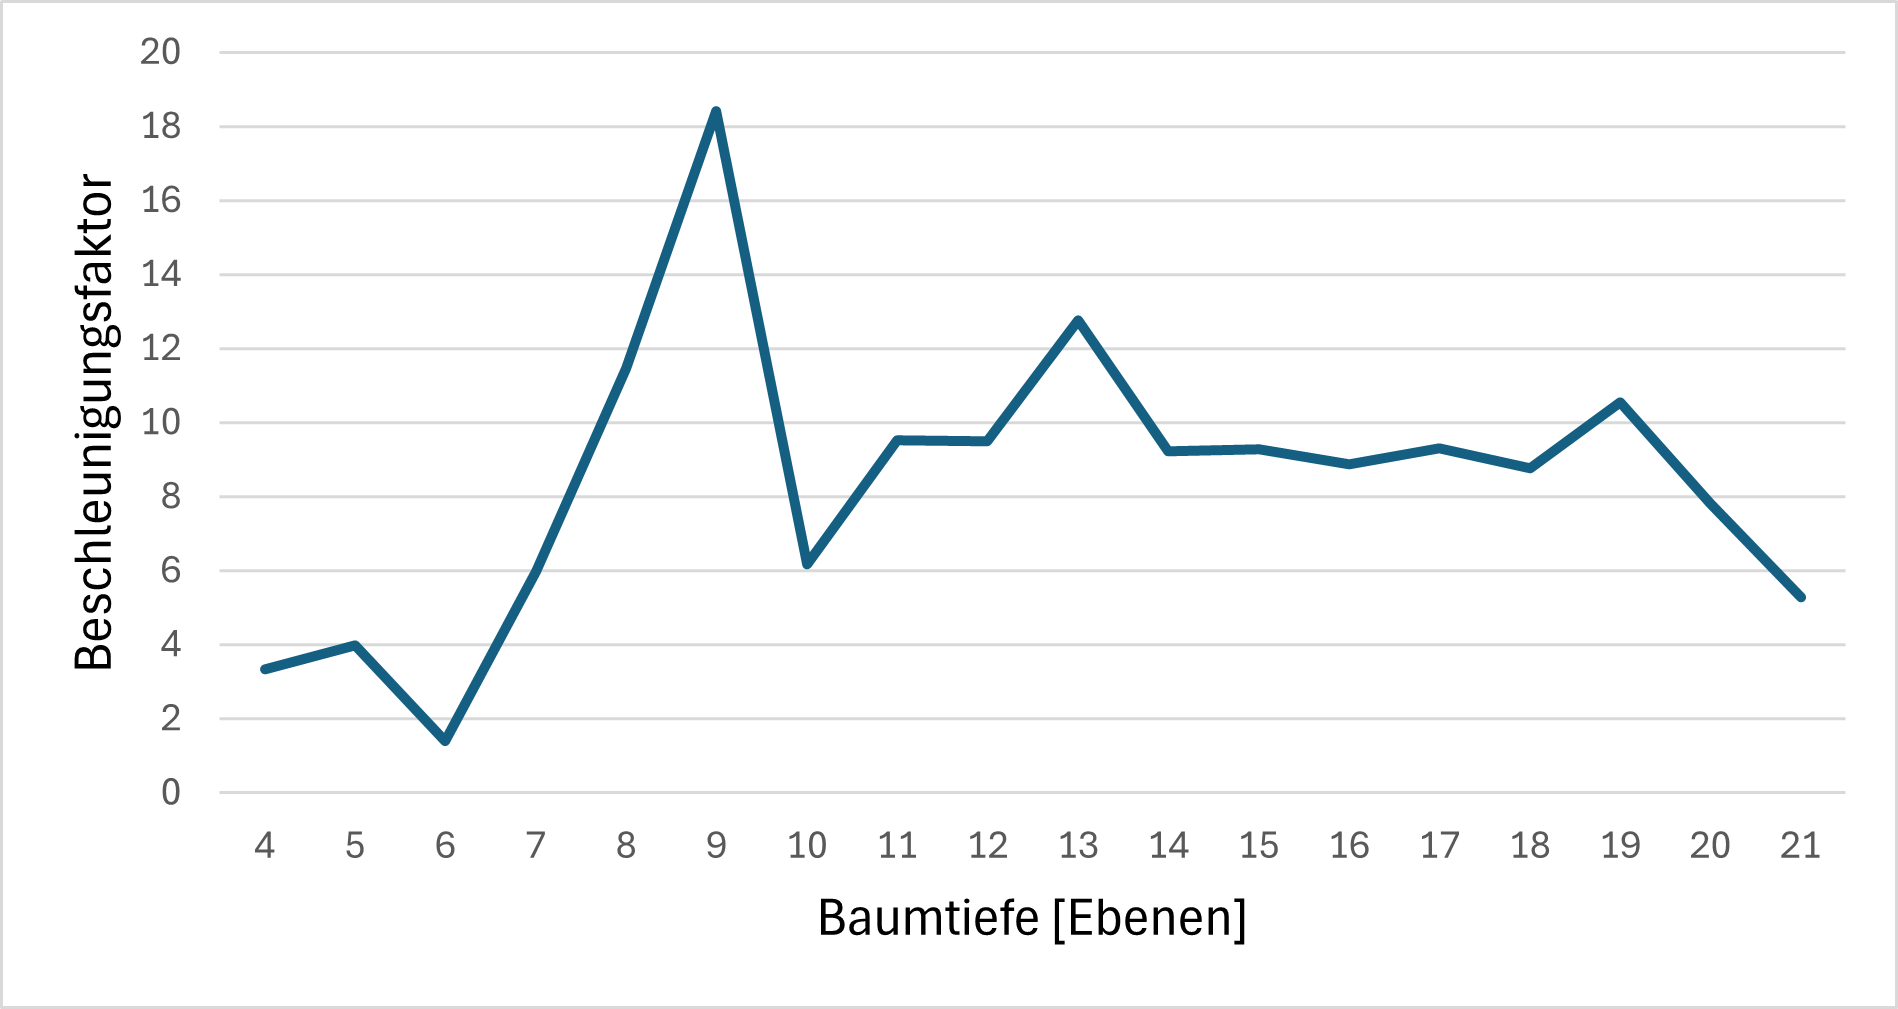
\includegraphics[width=\linewidth]{diagrams/Amdahl_Nvidia4096.png}
    \captionof{figure}{Beschleunigung nach Amdahl für verschiedene Baumtiefen auf Nvidia RTX A3000 mit 4096 Cores}
    \label{fig:AmdahlsLaw}
\end{minipage}
\hfill
\begin{minipage}{0.49\linewidth}
    \centering
    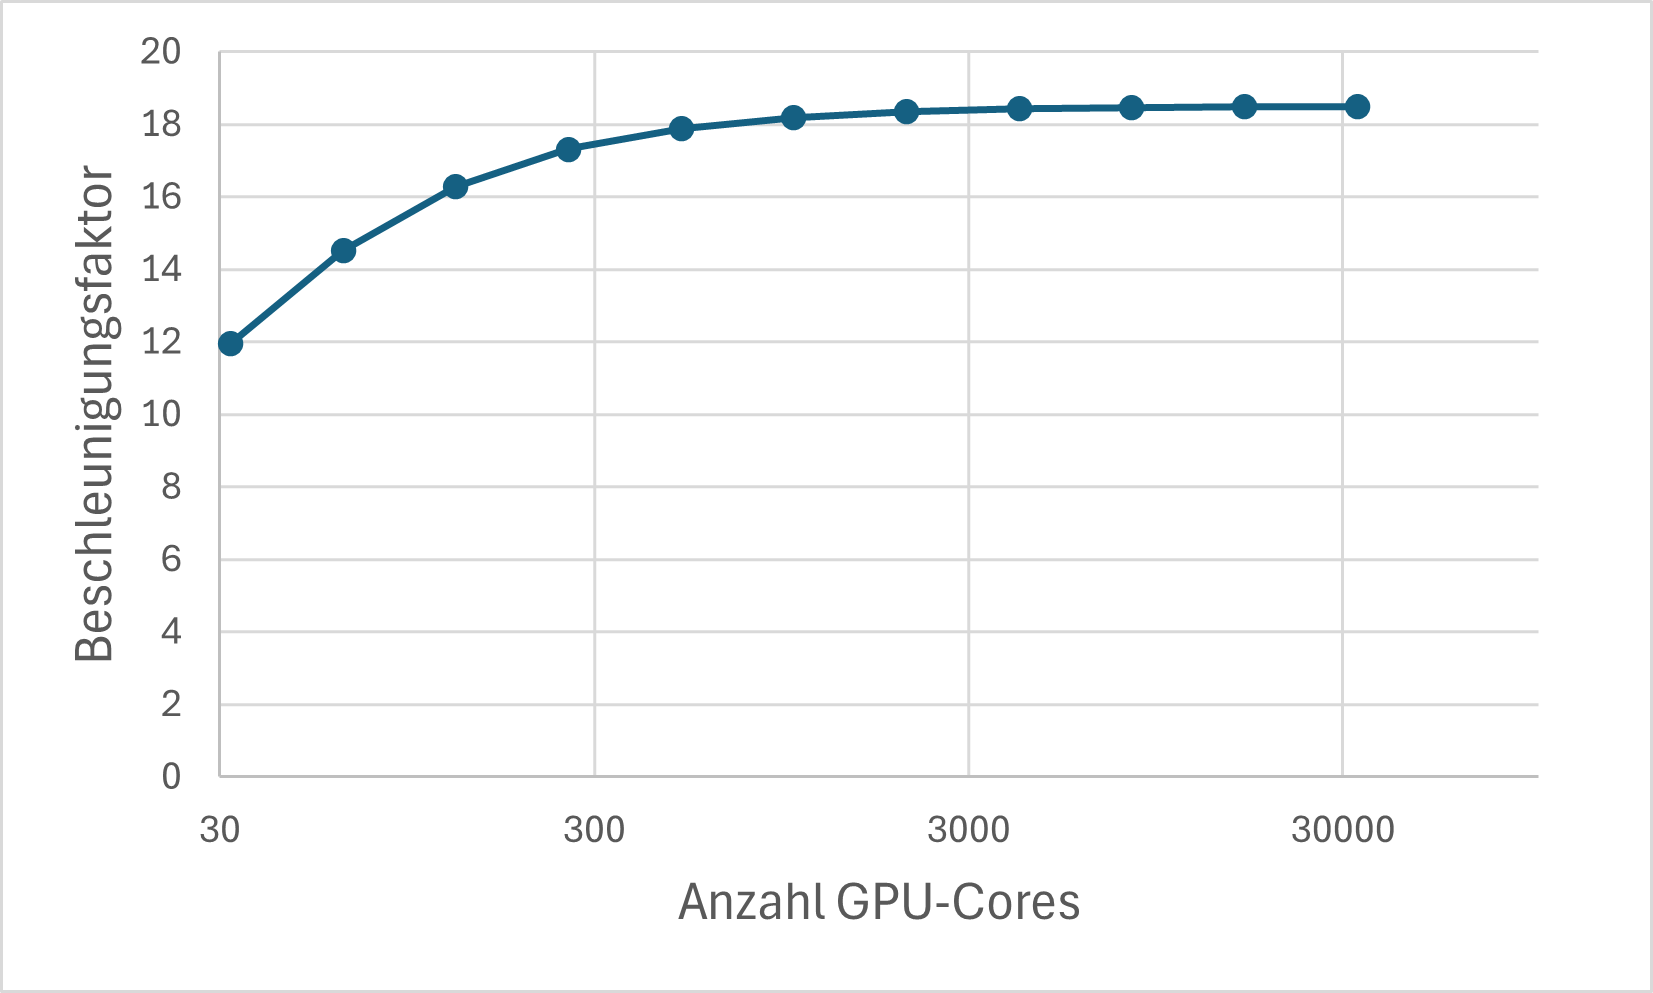
\includegraphics[width=\linewidth]{diagrams/Amdahl_maxBeschleunigung.png}
    \captionof{figure}{maximale Beschleunigung nach Amdahl auf Nvidia RTX A3000}
    \label{fig:AmdahlMaxBeschleunigung}
\end{minipage}

% ----------------------------------- Ansätze kombinieren ---------------------------------------
% -----------------------------------------------------------------------------------------------
\vspace{0.25cm}
\subsection{Kombinieren verschiedener Ansätze}\label{openCL-Fehler}
\vspace{-0.25cm}
Die mit den Ebenen steigende Komplexität unseres Programms hat einen großen Einfluss auf 
seine Gesamtlaufzeit. Für die ersten Ebenen bringen Parallelisierungen einen großen Overhead
mit sich, bei späteren Ebenen sind sie jedoch wesentlich schneller als die sequentielle Ausführung.\\
Zum Erreichen einer möglichst guten Programmlaufzeit entschlossen wir uns, die einzelnen 
Technologien kombiniert auszuführen. An welchen Stellen optimalerweise zwischen den Ansätzen
gewechselt werden sollte, ließ sich dabei gut aus den Schnittpunkten in den Laufzeit-Graphen ableiten. 
Diese sind zwar für jedes Endgerät unterschiedlich, können aber anhand unserer Erkenntnisse grob festgelegt werden.
\\Auf dem Thinkpad P15 konnten wir folgende Ergebnisse erzielen:
\begin{itemize}[itemsep=0pt, parsep=0pt, topsep=0pt, partopsep=0pt]
    \item Baum der Tiefe 24: ca. 17 Sekunden\\
            Ebenenverteilung: seriell 7 / OMP 16 / OCL 1 Ebenen
    \item Baum der Tiefe 24: ca. 10 Sekunden\\
            Ebenenverteilung: seriell 9 / OMP 15 Ebenen
    \item Baum der Tiefe 25: ca. 45 Sekunden\\
            Ebenenverteilung: seriell 9 / OMP 14 / OCL 2 Ebenen
\end{itemize}
Auf einem Desktop-PC wurden 24 Ebenen mit einer Verteilung von seriell 5 Ebenen, OpenMP 12 Ebenen und 
OpenCL 6 Ebenen als bestmögliche Baumtiefe in kürzestmöglicher Zeit  erreicht.
\vspace{0.25cm}\\
Im Rahmen unserer Analysen stießen wir auf zwei verschiedene Bottlenecks, welche beide an die Speicherkapazität
gebunden sind: 
Wie im folgenden Abschnitt \hyperref[Speicher]{5 Speicher} ausführlich evaluiert, wächst der Speicherplatzbedarf
für die Quader quadratisch. Daraus resultiert, dass Bäume mit mehr als 23 Ebenen in der Regel nicht generierbar sind.\\
Weiterhin tritt sofern man OpenCL mit großen Tiefen ausführt je nach Rechner zu unterschiedlichen Zeitpunkten 
der Fehlercode \texttt{-4 CL\_MEM\_OBJECT\_ALLOCATION\_FAILURE} auf, welcher auf nicht genügend verfügbaren Speicher
auf der GPU hindeutet. Diesen erhielten wir auf dem Thinkpad P15 ab der 26. Ebene und auf dem Thinkpad P14s ab der 24. Ebene. 